\chapter{Материал и методика}
	\section{География исследований}
Географическое распространение вида {\it M.~balthica} охватывает бореальную зону Атлантического и Тихого океанов.
В Европеской части ареала {\it M.~balthica} заходит в арктические моря, и встречается в Норвежском, Баренцевом, Белом и Карском морях.
Наиболее северной точкой считается Шпицберген (\cite{Zacepin_Filatova_1968}).
Таким образом, Белое и Баренцево моря являются краевой частью ареала для маком.
		\subsection{Белое море}
В вершине Кандалакшского залива наблюдения проводили на $6$ участках в рамках работы экспедиций Группы исследований прибрежных сообществ Лаборатории экологии морского бентоса (гидробиологии) СПбГДТЮ (рис.~\ref{ris:karta_White}). 
	\begin{figure}[p]
    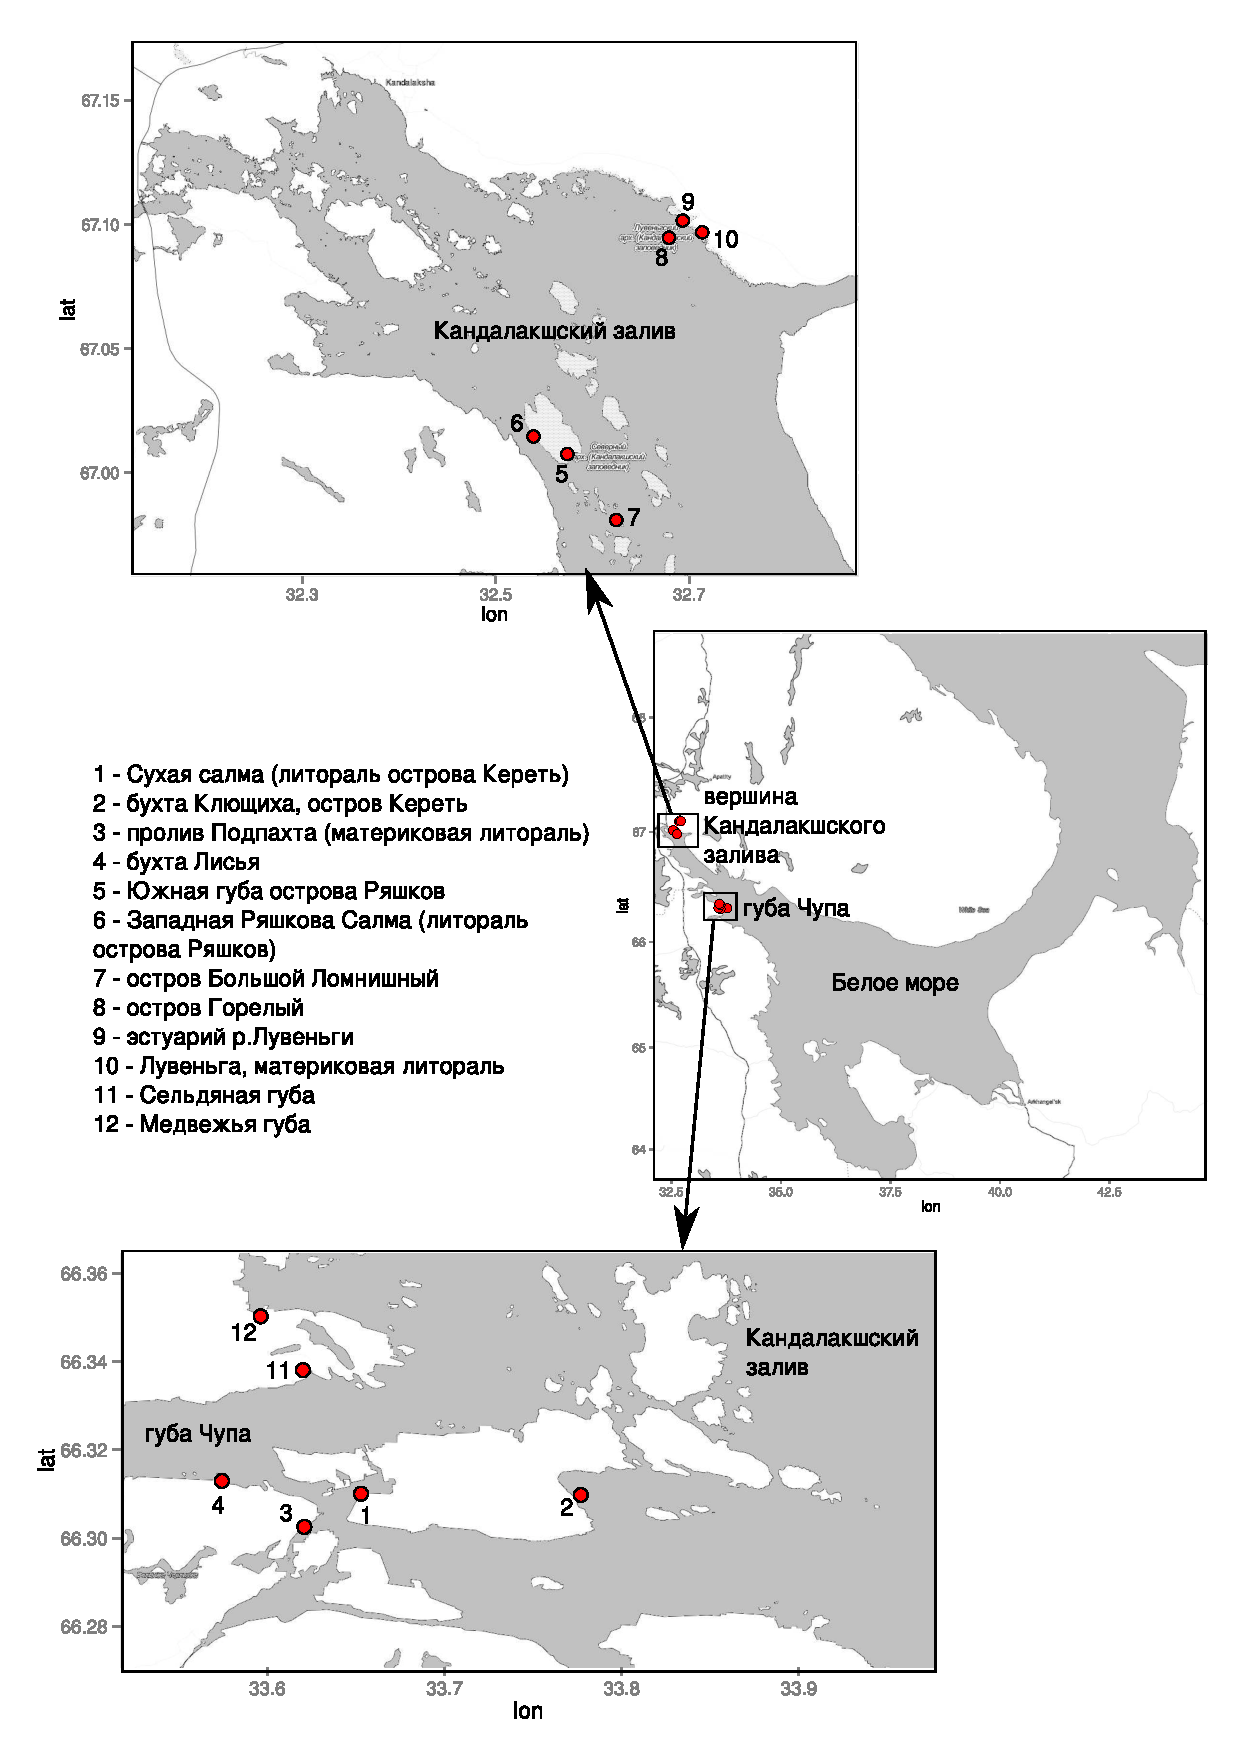
\includegraphics[width=\textwidth]{../maps/White_sea1.pdf}
    \caption{Исследованные участки в Кандалакшском заливе Белого моря}
    \label{ris:karta_White}
	\end{figure}
Три участка расположены в районе Лувеньгских шхер: эстуарий реки Лувеньги, Илистая губа острова Горелого и участок материковой литорали в $800$ метрах западнее поселка Лувеньга (участки 1, 2 и 3).
Один участок был расположен на литорали острова Ряшков в Западной Ряшковой Салме (Северный архипелаг) (участок 4).
В работе использованы данные Д.\:А.~Аристова из Южной губы о.~Ряшков и с о.~Большой Ломнишный (Северный архипелаг) (рис.~\ref{ris:karta_White}, участки 5 и 6). 

В районе губы Чупа исследования проводили на $4$ участках (рис.~\ref{ris:karta_White}) в ходе экспедиций кафедры ихтиологии и гидробиологии СПбГУ. 
Два участка были расположены на литорали острова Кереть --- в Сухой Салме и бухте Клющиха (участки 7 и 8). 
Один участок был расположен на материковой литорали пролива Подпахта и один --- в бухте Лисьей (участки 9 и 10).

%Также в работе использованы данные ББС <<Картеш>> ЗИН РАН по обилию маком в губах Медвежья и Сельдяная (\cite{Varfolomeeva_Naumov_2013}) (рис.~\ref{ris:karta_White}, участки 11 и 12).

\afterpage{\clearpage}

		\subsection{Баренцево море}
Материал  в акватории Баренцева моря  был  собран    в ходе   студенческой баренцевоморской экспедиции СПбГУ. 
Всего было исследовано $8$ участков --- $2$ в Кольском заливе и   $6$  в   прибрежной   зоне  Восточного  Мурмана (рис.~\ref{ris:karta_Barents}).  
	\begin{figure}[p]
    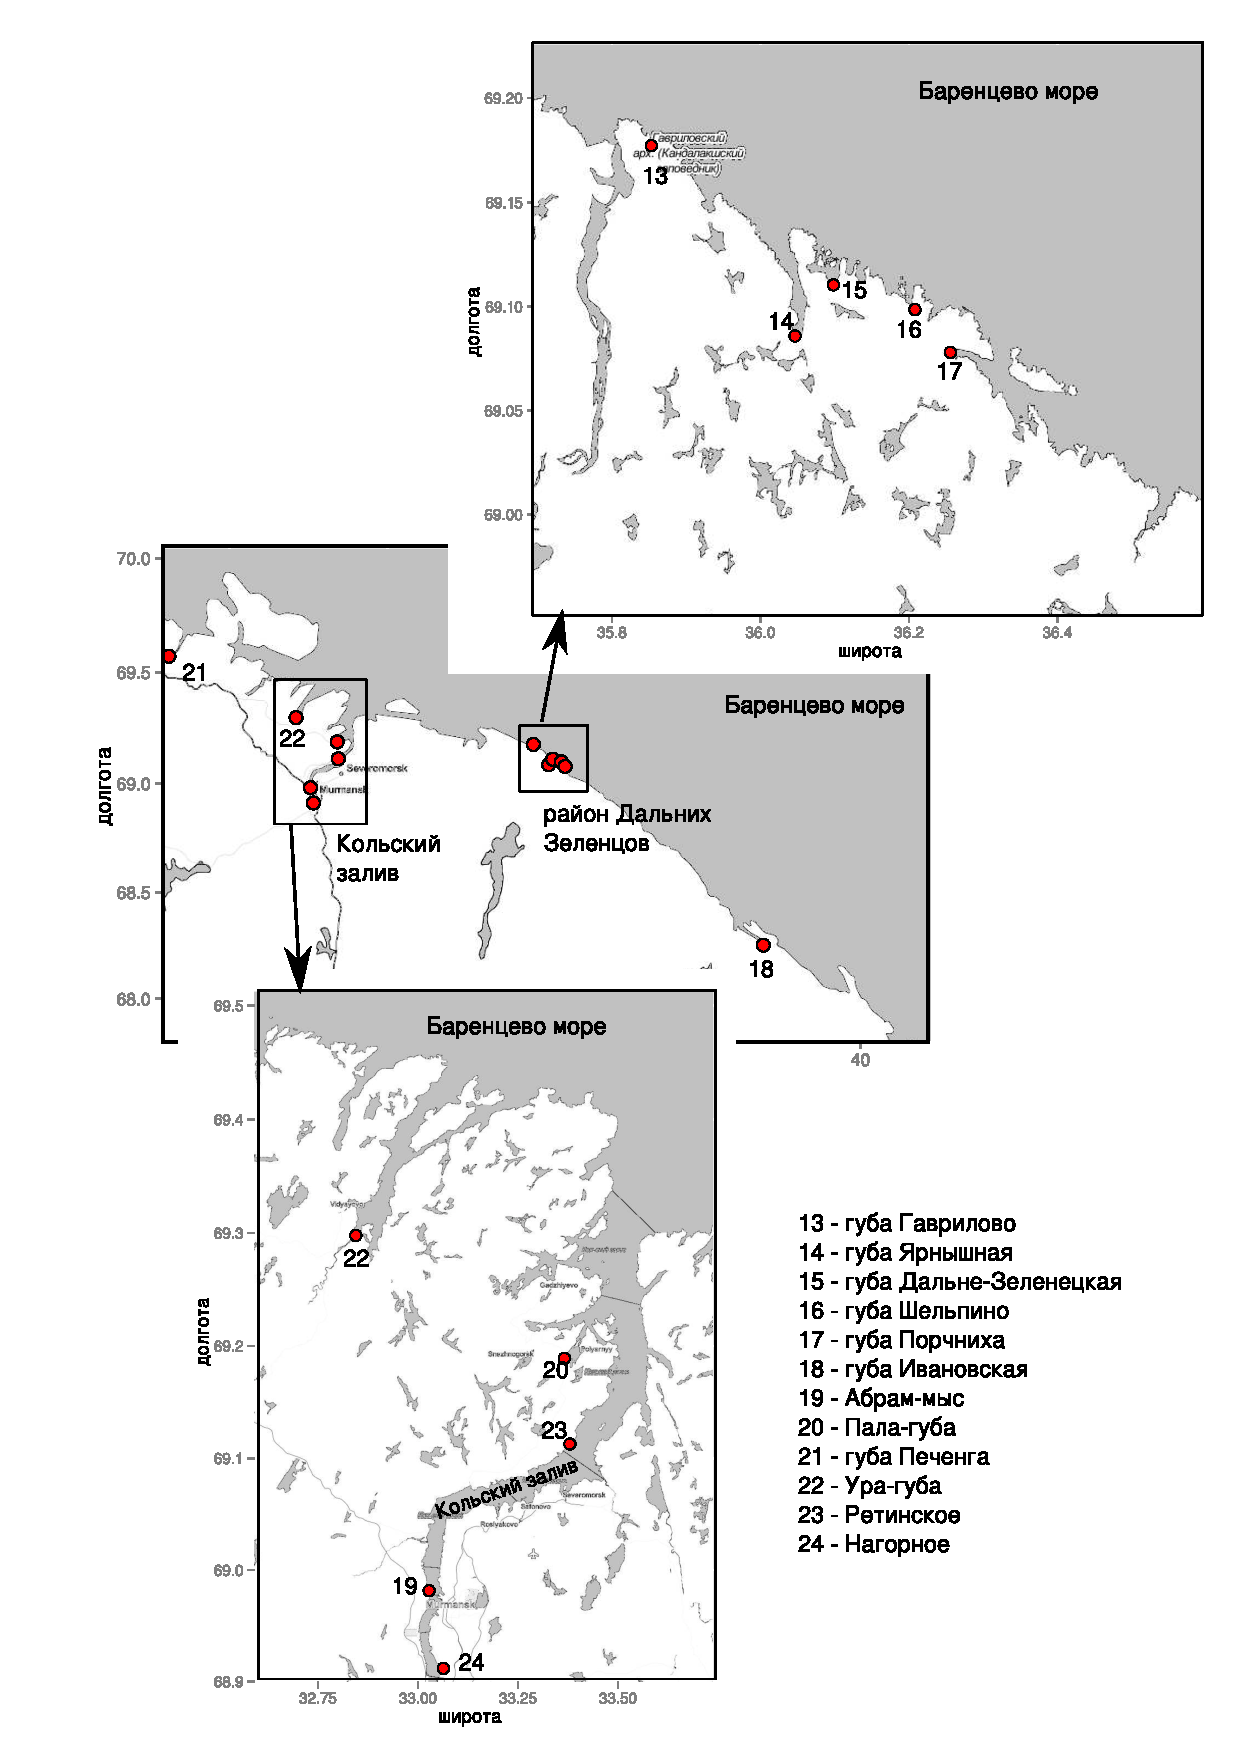
\includegraphics[width=\textwidth]{../maps/Barents_sea1.pdf}
    \caption{Исследованные участки вдоль Мурманского побережья Баренцева моря}
    \label{ris:karta_Barents}
	\end{figure}
На   Восточном   Мурмане исследованные участки литорали  были   расположены   в   губах   Гавриловская (участок 13),  Ярнышная (участок 14), Дальнезеленецкая (участок 15), Шельпинская (участок 16), Порчниха (участок 17) и Ивановская (участок 18).
Участки литорали  в   Кольском   заливе   были  расположены на побережье в районе Абрам-мыса (участок 19) и в Палa-губе (участок 20), в районе города Полярный. 


Также в работе использованы данные К.\:В.~Шунькиной и Е.\:А.~Генельт-Яновского по обилию маком в губе Печенга и Ура-губе (Западный Мурман) (рис.~\ref{ris:karta_Barents}, участки 21 и 22), и в районе Северного Нагорного и Ретинского (Кольский залив) (рис.~\ref{ris:karta_Barents}, участки 23 и 24).

\afterpage{\clearpage}

    \section{Характеристика местообитаний}
Для всех участков было составлено физиономическое описание.
На каждом участке измеряли ширину литорали.
По горизонтам описывали визуально тип грунта, наличие валунов, бурых водорослей, взморника \textit{Zostera marina}, зеленых нитчатых водорослей. 
Также описывали поясность сообществ, если она была выражена.
Термогалинные характеристики для отдельных участков не были описаны, и мы использовали литературные данные о среднегодовых параметрах для акваторий, и опубликованные данные о динамике температур в исследованный период.
Подробное описание данных характеристик приведено в главе Обсуждение результатов.

Показательной комплексной оценкой гидродинамики региона и условий питания детритофагов служат показатели состава грунта. 
Поэтому на ряде исследованных участков были отобраны образцы грунта. 
В Белом море грунт исследовали на обоих участках в губе Чупа и на трех участках в вершине Кандалакшского залива.
В Баренцевом море грунт исследовали на всех участках Восточного Мурмана и двух участках Кольского залива (Абрам-мыс и Пала-губа).

Пробы грунта отбирали на всех исследованных горизонтах каждого участка.
В экспедиции после отбора из грунта выбирали крупных животных (червей, раков, моллюсков, приапулид), образцы высушивали и упаковывали для отправки в город. 
В городе образцы досушивали в термостате при температуре $105^o$C до момента, когда масса образца переставала изменяться. 
Из каждого образца брали по три навески грунта для определения содержания органических веществ. 
Навески помещали в муфельную печь с температурой $450^o$C на $8$ часов. 
После сжигания навески повторно взвешивали, и по разнице масс определяли массовую долю органических веществ в грунте. 
По трем навескам рассчитывали среднюю массовую долю для каждого образца.

Оставшийся грунт использовали для определения гранулометрического состава. 
При описании гранулометрического состава грунта использовали классификацию И.\,Л.~Безрукова и А.\,Н.,~Лисицина для морских водоемов (таблица~\ref{tab:lisicyn_granulometriya}, \cite{Bezrukov_Lisicyn_1960}).
\begin{table}[p]
    \centering
    \caption{Классификация фракций грунта по размеру частиц (\cite{Bezrukov_Lisicyn_1960})}
    \label{tab:lisicyn_granulometriya}
\begin{tabular}{|l|l|}
    \hline
    Размер фракции,~мм & Название фракции         \\ \hline
     $> 10$    & Крупный и средний гравий  \\
    $10-5$               & Мелкий гравий         \\
    $5-3$                & Очень мелкий гравий   \\
    $3-1$                & Очень крупный песок   \\
    $1-0,5$              & Крупный песок         \\
    $0,5-0,25$           & Средний песок         \\
    $0,25-0,1$           & Мелкий песок          \\
    $< 0,1$           & алевриты       \\\hline
\end{tabular}
\end{table}
Для этого грунт взвешивали, после чего просеивали в сухом состоянии через колонку сит (диаметр ячеи: $10 - 5 - 3 - 1 - 0,5 - 0,25$~мм). 
Частицы размером менее $0,25$~мм просеивали через сито с диаметром ячеи $0,1$~мм с использованием струи воды, после чего оставшиеся на сите --- высушивали при температуре $105^o$C. 
Каждую фракцию частиц взвешивали, и определяли их массовую долю. 
Анализ частиц размером менее $0,1$~мм (алевритов)не проводили. 

\afterpage{\clearpage}

    \section{Описание сообществ, включающих {\it Macoma balthica}}
На 6 мониторинговых участках в Кандалакшском заливе Белого моря проводили качественное описание фауны в пределах обследованных горизонтов литорали.
Таким образом, всего составлено $12$~описаний.
На каждом участке в акватории Баренцева моря исследовали все  горизонты литорали, представленные мягкими грунтами.  
Таким образом, всего было составлено $16$ описаний.

Как основное орудие сбора использовали литоральную рамку площадью $1/30$~м$^2$, из которой изымали грунт на глубину $5$~см. 
В случае, когда приходилось отбирать пробы из-под воды, использовали зубчатый водолазный дночерпатель площадью захвата $1/20$~м$^2$.
Отобранные пробы промывали на сите с диаметром ячеи $1$~мм. 

После промывки из   проб   выбирали   всех   особей  {\it M.~balthica}  и   представителей   сопутствующего макрозообентоса    для   определения   состава   сообщества.
Представителей   сопутствующего макрозообентоса  определяли   до   минимально   возможного   таксона. Таксономию и номенклатуру сверяли по Всемирному регистру морских видов (\cite{WoRMS}).

Для сравнения видового состава сообщества использовали коэффициент Жаккара. 
Результаты визуализировали при помощи  кластерного анализа методом ближайшего соседа. 
Достоверность выделенных групп оценивали с помощью анализа сходства профилей (SIMPROF) (\cite{Clarke_et_al_2008}).
Для оценки влияния факторов использовали многомерное шкалирование MDS в сочетании с анализом сходства ANOSIM.
Анализы проводили в программе PaSt (\cite{Hammer_et_al_2001}) и \R{} (\cite{R_2014}).


%	\subsection{Изучение микрораспределения {\it Macoma balthica}}

%\textcolor{red}{квадраты на Белом}

%\textcolor{red}{квадраты на Баренцевом}
%При оценке распределения особей в губе Порчниха в 2007 г. было отобрано 32 пробы рамкой 1/30м2, причем пробы брались вплотную друг к другу 4 рядами по 8 шт.

% из Генельт-Кобылков-Назарова, 2007 (что это было??)
%Изучение распределения особей {\it Macoma baltica} было проведено в Баренцевом море по методике, описанной Трашем (\cite{Thrush_et_al_1989}) с изменением масштаба.
%Исследования были проведены в августе $2007$~г. на илисто-песчаной литорали кутовых участков губ Восточного Мурмана --- Ярнышной и Дальнезеленецкой, и в октябре $2007$~г. на литорали Пала-губы (Кольский залив). 
%Для Дальнезеленецкой губы съемка была повторена в августе $2008$ года на полигоне двойного размера.

%В каждой точке отбиралось по $36$ проб площадью $1/30$~м$^2$, расположенных в пределах участка размером $7,5 \times 12$~м. 
%Координаты каждой пробы были определены в декартовой системе координат в метрах, один из углов участка служил точкой отсчета. 
%В дальнейшем пробы промывали на сите с диаметром ячеи $1$~мм. 
%В лаборатории были выбраны и  подсчитаны все макомы.

%При дальнейшей обработке данных для каждого участках подсчитывали индекс структурности (отношение дисперсии к средней арифметической). 
%Для анализа размеров агрегаций были построены коррелограммы, основанные на коэффициенте пространственной автокорреляции Морана (\cite{ncf}).
%Достоверность коэффициентов определяли пермутационным методом.
%Наличие градиентов проверяли с использованием корреляционного анализа Кендалла между координатами проб и обилием вида в каждой пробе. 
%Все статистические анализы проводили в статистической среде \R{} (\cite{R_2014}) с $95\%$ доверительной вероятностью ($P < 0,05$).
%Для интерпретации результатов корреляционного анализа были использовали пузырькоые диаграммы.

\afterpage{\clearpage}	

	\section{Изучение структуры поселений {\it Macoma balthica}}
Для описания структуры поселений использовали данные всех доступных сборов.

В Белом море всего было обследовано $10$ участков в акватории Кандалакшского залива. 
На шести из них наблюдения проводили на всех горизонтах литорали, представленных мякими грунтами.
На четырех других были обследованы отдельные горизонты. 

Для Баренцева моря были использованы данные по обилию с $12$ участков. 
На каждом участке в акватории Баренцева моря исследовали все  горизонты литорали, представленные мягкими грунтами.  

Как основное орудие сбора использовали литоральную рамку площадью $1/30$~м$^2$, из которой изымали грунт на глубину $5$~см. 
В случае, когда приходилось отбирать пробы из-под воды, использовали зубчатый водолазный дночерпатель площадью захвата $1/20$~м2.
Отобранные пробы промывали на сите с диаметром ячеи $1$~мм или $0,5$ (на трех мониторинговых участках в районе Лувеньги и в Западной Ряшковой Салме, участки $7, 8 - 10$ на рис.~\ref{ris:karta_White}). 
После промывки из   проб   выбирали   всех   особей  {\it M.~balthica}.
Подробная информация о количестве проб и размере учетных площадок для каждого участка представлены в приложении~\ref{app:NB_table}.

В дальнейшем подсчитывали количество особей в пробах, которое пересчитывали в численность моллюсков на квадратный метр. 
Для всех средних значений расчитывали точность учета $d,\% = m/M$, где $m$~--- стандартная ошибка средней, $M$~--- средняя арифметическая.
Биомассу определяли путем взвешивания на весах с точностью 10 мг, либо, для части участков на Белом море, рассчетным методом.
Мы использовали формулу зависимости массы макомы от ее длины $W = 0,00016 \times L^{2,96}$, полученную для губы Чупа (\cite{Maximovich_et_al_1993}).


Изучение размерной структуры поселений маком проводили на всех участках.
Для этого у всех моллюсков в пробах под бинокуляром измеряли максимальный линейный размер (длину) с точностью $0,1$~мм.
По полученным данным строили размерно-частотное распределение с шагом $1$~мм.

%Кроме того, на части участков у моллюсков подсчитывали количество меток зимней остановки роста, которое принимали как возраст моллюсков --- число прожитых зим (например, $4+$ это  особи возрастом от $4$ до $5$ лет).   
%Таким   образом   были   получены   оценки возрастной структуры поселений {\it M. balthica}.

Для визуализации данных по обилию использовали графики Тьюки (Tukey boxplots, \cite{Tukey_1977}). 
Сравнение обилия проводили с помощью непараметрического теста Краскел-Уоллиса. 
Для выявления связи величин обилия с гранулометрическим составом грунта использовали непараметрическую корреляцию Спирмена (\cite{Hollander_et_al_2013}).
Классификацию размерных структур проводили с помощью анализа главных компонент (\cite{Mardia_et_al_1979}).
Все анализа проводили в статистической среде \R{} (\cite{R_2014}).

\afterpage{\clearpage}

	\section{Изучение динамики поселений {\it Macoma balthica}}
        \subsection{Белое море}
В Белом море динамику поселений {\it Macoma balthica} исследовали на $6$ участках в районе вершины Кандалакшского залива. 

Сборы проводили с 1992 по 2012 год ежегодно в июле-августе.
Автор принимала участие в полевых сборах с $1999$ по $2007$ год.
Данные за другие годы взяты из архива ГИПС ЛЭМБ.

Структура материала представлена в таблице \ref{tab:material_Kandalaksha}.
\begin{table}[p]
\caption{Структура материала по динамике поселений {\it Macoma balthica} вершины Кандалакшского залива}
\label{tab:material_Kandalaksha}
%\begin{tabular}{|*{5}{p{0.2\textwidth}|}} \hline
    \begin{tabularx}{\textwidth}{|*{5}{X|}} \hline
участок & годы наблюдения & обследованные горизонты литорали & количество проб в однократной съемке & площадь пробоотборника, м$^2$  \\ \hline
о. Горелый Лувеньгских шхер & 1992 -- 2012 & ВГЛ, СГЛ, НГЛ & 1-3 & 1/30, 1/10 \\ \hline
Материковая литораль в районе пос. Лувеньга & 1992-2000, 2002, 2004 & ВГЛ, СГЛ, НГЛ & 12-20 & 1/30 \\ \hline
Эстуарий р. Лувеньги & 1992 -- 2012 & СГЛ & 3 & 1/10 \\ \hline
Литораль Западной Ряшковой Салмы о. Ряшкова & 1994 -- 2012 & СГЛ & 2 & 1/10 \\ \hline
Южная губа о. Ряшкова & 2001 -- 2012 & НГЛ & 9-16 & 1/30 \\ \hline
о. Ломнишный & 2007 -- 2012 & НГЛ & 5-10 & 1/30  \\ \hline
\end{tabularx}
\end{table}

На каждом исследованном участке отбирали $3 - 25$ проб площадью $1/30 - 1/10$~м$^2$, которые затем промывали на сите с диаметром ячеи $0,5 - 1$~мм. 
В пробах учитывали всех особей {\it M.~balthica}, у которых в дальнейшем измеряли максимальный линейный размер (длину) с точностью ~0,1~мм. 

Для определения биомассы моллюсков взвешивали на электронных весах с точностью до $1$~мг. 
Для серий проб, где не проводили взвешивание моллюсков, биомассу определяли рассчетным методом с использованием аллометриеской зависимости сырой массы маком от длины их раковины (\cite{Maximovich_et_al_1993}). 

В дальнейшем рассчитывали показатели средней численности маком на квадратный метр (плотность поселения) и размерно-частотное распределение особоей.
Для построения размерно-частотного распределения шаг размерного класса составлял $1$~мм.

В дальнейшем при анализе мы работали с особями с длиной раковины более $1,0$~мм по двум причинам. 
Во-первых, для того чтобы сделать сравнимыми результаты с разных участков, где пробы промывались на ситах с разным диаметром ячеи. 
Во-вторых, пробы отбирали в середине лета, то есть к этому моменту молодь этого года частично осела, то есть оценка численности данной группы будет некорректна.
Мы считаем корректной такую редукцию материала, поскольку для Белого моря считается, что усешность пополнения поселений молодью в первую очередь зависит от выживаемости спата зимой (\cite{Maximovich_Gerasimova_2004}).

Для анализа динамики пополнения поселений молодью в $2012 - 2013$ годах у особей длиной менее $3$~мм были измерены длины колец зимней остановки роста. 
После определения размеров годовалых особей, по размерной было рассчитано их обилие в каждом году мониторингового наблюдения.
Всего было промерено 496 особей.



В работе использованы мониторинговые данные кафедры ихтиологии и гидробиологии СПбГУ по обоим участкам на острове Кереть (\cite{Maximovich_et_al_1991, Gerasimova_Maximovich_2013}) (рис.~\ref{ris:karta_White}, участки $1, 2$). 
Также в работе использованы многолетие данные ББС <<Картеш>> ЗИН РАН по обилию маком в губах Медвежья и Сельдяная (\cite{Varfolomeeva_Naumov_2013}) (рис.~\ref{ris:karta_White}, участки $11, 12$).


 
%методика из Назаровой-Полоскина
%Материал собран в августе 1992 - 2003 гг. Изучено три литоральных поселения маком: в Илистой губе острова Горелого (участок 1), в эстуарии реки Лувеньги (участок 2) и на материковой литорали к югу от поселка Лувеньга (участок 3). Сборы проведены пробоотборником площадью захвата 1/30 м2. Разовая выборка составляла от 9 до 25 проб с участка. Грунт выбирался до глубины 5 см и промывался на сите с диаметром ячеи 0.5мм.  Всех особей  M. balthica измеряли с точностью 0.1 мм. В каждый момент наблюдений определяли размерную структуру и плотность поселения маком. 



% методика из Аристова
%Оба участка закрыты от волнового воздейст-
%вия. Литораль в районе исследований представляет собой песчаный пляж с примесью
%ила с вкраплениями крупных валунов. Спуск в сублитораль пологий, отчетливо вы-
%раженный пояс фукоидов отсутствует. Население представлено типичными формами,
%такими как Arenicola marina, Macoma balthica, Mya arenaria, Hydrobia ulvae, Microspio sp.
%и др. (Д. А. Аристов, неопубликованные данные).
%В обеих точках производили сборы по следующей методике: в районе нуля глубин
%во время отлива в пределах участков случайным образом выбирали и обследовали не-
%сколько площадок. Поскольку радиусы индивидуальной активности A. islandica и пред-
%полагаемых жертв (двустворчатых моллюсков) существенно различаются, в пределах
%каждой площадки брали пару проб методом вложенных рамок. Первую пробу из пары
%(1/4 м2) брали для учета A. islandica. Грунт из пробы тщательно перебирали вручную,
%всех найденных представителей сем. Naticidae подсчитывали и определяли их видовую
%принадлежность. Вторая проба (1/30 м2) была взята для учета потенциальных жертв —
%двустворчатых моллюсков. Грунт из нее промывали на сите с диаметром ячеи 1 мм,
%а затем остаток разбирали в фотографической кювете с белым дном. Из грунта соби

\afterpage{\clearpage}

        \subsection{Баренцево море}
% из Дерюгинских, 2007 + новой статьи

В Баренцевом море динамику поселений маком исследовали на модельном участке --- литоральной отмели Дальний пляж губы Дальнезеленецкой. 
В работе использованы материалы экспедиции по мониторингу Дальнего пляжа губы Дальнезеленецкой с $2002$ года, любезно предоставленные Е.\:А.~Генельт-Яновским.
Автор принимала участие в полевых сборах в $2006 - 2008$~гг.

Материал был собран в июле-августе $2002 - 2008$~гг. в пределах от верхнего горизонта песчаной литорали ($+2,0$~м) до $+0,7$~м над нулем глубин. 

 В $2002$ году была заложена сетка из $8$ станций. 
 В пределах каждой станции отбирали $3 - 5$ проб площадью $1/10$~м$^2$, которые промывали на сите с диаметром ячеи $1$~мм. 
 У всех двустворчатых моллюсков измеряли длину раковины с точностью $0,1$~мм. 
 С 2004 года отбирали пробы на трех станциях из $8$, которые располагались в контрастных сообществах (\cite{Genelt_Dalnezeleneckaya_2008}). 

В качестве точки сравнения нами был выбран $1973$ год (\cite{Streltsov_et_al_1974, Agarova_et_al_1976}), поскольку в тот год была проведена основная количественная съемка на Дальнем пляже. 

 %Восстановление возрастной структуры {\it Macoma balthica} для 2002-06 годов было проведено по моллюскам из выборки 2007 года. Для этого у них были измерены кольца зимней остановки роста и рассчитаны размеры моллюсков каждой возрастной группы. В качестве границ размерно-возрастных классов принималась середина соответствующего размерного диапазона. В дальнейшем, в зависимости от длины, каждого моллюска из выборок 2002-06 гг. относили к определенному возрастному классу. Так как в 2007 году не были встречены особи с 8 видимыми кольцами зимней остановки роста, то все особи крупнее 17,7 мм (верхняя размерная граница возрастного класса 8+) были объединены в одну группу.

Сравнение средних проводили с помощью критериев Вилкоксона и Краскел-Уоллеса (\cite{Hollander_et_al_2013}).
При анализе трендов в динамике поселений использовали корреляционный анализ Мантеля (\cite{Legendre_Legendre_2012}) для удаления тренда из рядов. 
Также данный метод использовали для оценки синхронности динамик обилия моллюсков в разных поселениях.
Для выяления плотностнозависимых процессов были использованы частные автокорреляции (PRCF --- Partial rate correlation function) (\cite{Berryman_Turchin_2001}).
Для изучения влияния температуры на динамику обилия \textit{M.~balthica} использовали линейные модели (\cite{Chambers_Hastie_1991}).
Оценку корректности построенной модели проверяли с помощью критериев Дарбина-Уотсона (отсутствие автокорреляций), Шапиро-Уилка (нормальное распределение остатков) и Бройше-Пагана (гомогенность дисперсий).
Все рассчеты проводили в статистической среде \R{} (\cite{R_2014}).

\afterpage{\clearpage}

	\section{Изучение линейного роста {\it Macoma balthica}}
%из статьи про рост
Рост \textit{M.~balthica} в Белом море достаточно детально изучен (\cite{Semenova_1970, Maximovich_et_al_1992, Hummel_et_al_1998}), поэтому мы проводили специальные исследования только для Баренцева моря.

Рост изучали по материалам, полученным в августе $2007 - 2008$~гг. для $7$ участков в Баренцевом море: Абрам-мыс, Пала-губа, губы Гавриловская, Ярнышная, Дальнезеленецкая, Шельпино, Порчниха.
Станции для отбора проб располагали по горизонтам литорали. 

У всех особей {\it Macoma balthica} в пробах ($1/30$ или $1/20$~м$^2$, промывка на сите с диаметром ячеи 1~мм) измеряли длину (наибольший линейный размер) раковины и (по меткам роста) ее значения в период каждой зимней остановки роста с точностью 0,1 мм.
Полученные для каждой станции измерения особей были сведены в описание возрастной структуры по схеме, представленной в табл.~\ref{tab:rost_matrica_primer}. 
\begin{table}[p]
        \caption{Пример треугольной матрицы с данными по росту моллюсков и их возрастной структуре}
        \label{tab:rost_matrica_primer}
%    \begin{tabular}{|c|c|cc|cc|ccccccccc|}
        \begin{tabularx}{\textwidth}{|X|X|XX|XX|XXXXXXXXX|}
        \hline
        &    & \multicolumn{4}{c|}{$L$}               & \multicolumn{9}{c|}{$L_{k}$} \\ 
        $t$     & $N$  & $min$ & $max$ & $aver$ & $m_{L}$   & 1 к & 2к  & 3к  & 4к  & 5к  & 6к  & 7к  & 8к   & 9к   \\ \hline
        0+      & 0  &       &       &         &         &     &     &     &     &     &     &     &      &      \\
        1+      & 9  & 1,8   & 2,5   & 2,2     & 0,1     & 1,1 &     &     &     &     &     &     &      &      \\
        2+      & 76 & 1,6   & 7,9   & 3,1     & 0,1     &\cellcolor{yellow}0,7 & \cellcolor{yellow}2,0 &     &     &     &     &     &      &      \\
        3+      & 40 & 2,1   & 5,8   & 3,8     & 0,1     & 0,7 & 1,8 & 2,9 &     &     &     &     &      &      \\
        4+      & 34 & 2,1   & 8,5   & 5,4     & 0,2     & 0,7 & 1,8 & 3,1 & 4,6 &     &     &     &      &      \\
        5+      & 37 & 3,5   & 9,8   & 6,8     & 0,2     & 0,8 & 1,9 & 3,1 & 4,6 & 6,2 &     &     &      &      \\
        6+      & 44 & 4,6   & 11,5  & 8,2     & 0,2     & 0,8 & 1,8 & 2,9 & 4,1 & 5,5 & 7,3 &     &      &      \\
        7+      & 48 & 7,4   & 12    & 9,9     & 0,2     & 0,9 & 2,1 & 3,3 & 4,6 & 6,0 & 7,7 & 9,1 &      &      \\
        8+      & 61 & 8     & 13,7  & 10,6    & 0,1     & \cellcolor{red}0,7 & \cellcolor{red}2,0 & \cellcolor{red}3,4 & \cellcolor{red}4,6 & \cellcolor{red}6,1 & \cellcolor{red}7,5 & \cellcolor{red}8,9 & \cellcolor{red}9,9  &      \\
        9+      & 44 & 8,6   & 14,2  & 11,1    & 0,2     & -   & -   & 3,4 & 4,7 & 6,5 & 8,2 & 9,7 & 10,5 & 11,4 \\ \hline
                &    &       &       & $L_{k} aver$  &  & \cellcolor{blue}0,8 & \cellcolor{blue}1,9 & \cellcolor{blue}3,1 & \cellcolor{blue}4,5 & \cellcolor{blue}6,0 & \cellcolor{blue}7,7 & \cellcolor{blue}9,2 & \cellcolor{blue}10,2 & \cellcolor{blue}11,4 \\
                &    &       &       & $m_{Lк}$      &  & 0,0 & 0,0 & 0,1 & 0,1 & 0,2 & 0,2 & 0,3 & 0,4  &      \\
                &    &       &       & $L_{k} min$  &   & 0,7 & 1,8 & 2,9 & 4,1 & 5,5 & 7,3 & 8,9 & 9,9  &      \\
                &    &       &       &  $L_{k} max$ &   & 1,1 & 2,1 & 3,4 & 4,7 & 6,5 & 8,2 & 9,7 & 10,5 &     \\ \hline
    \end{tabularx}
    \footnotesize{Примечания: $t$ --- возраст моллюсков; 
        $N$ --- количество  особей  данного возраста, экз.; 
        $L min$  ---  минимальная   длина  особей   данного   возраста,   мм;   
        $L max$   ---   максимальная   длина   особей   данного   возраста,   мм; 
        $L aver$ --- средняя длина моллюсков данного возраста, мм; 
        $m_L$ --- ошибка средней, 
        $L_k$ 1к -- 13к --- длина особи к определенному возрасту, измеренная по меткам зимней остановки роста, мм;
        $L_k aver$ --- средняя длина данной метки остановки роста, мм; 
        $m_{L_k}$ --- ошибка средней; 
        $L_k min$ --- минимальная длина данной метки остановки роста, мм; 
        $L_k   max$   --   максимальная   длина   данной   метки   остановки   роста.   
        В   таблице   приведены средние длины данного кольца у моллюсков определенного возраста. \\[1em]
    Выделения: синий --- средневзвешенный возрастной ряд для маком в данном поселении;
        красный --- возрастной ряд отдельной генерации маком;
        желтый --- средний годовой прирост моллюсков в определнном возрасте}
\end{table}
Таким образом, всего было получено $14$ описаний, условно характеризующих отдельные поселения маком. 
Как видно из данных табл.~\ref{tab:rost_matrica_primer}, каждое из описаний содержало результаты реконструкции динамики средней длины раковины маком в генерациях. 
Эти данные мы использовали для сравнительного анализа характера линейного роста моллюсков в поселениях и расчета величин группового годового прироста особей в генерации (как разность средних длин раковин моллюсков в последовательные моменты зимней остановки роста).

Возрастные ряды аппроксимировали при помощи линейной модификации уравнения Берталанфи: $L_{t} = L_{max} \times (1 - e^{(-k(t - t_{0}))})$, где $L_{max}$, $k$, $t_{0}$ --- коэффициенты, $t$ --- возраст, а $L_{t}$ --- длина раковины моллюска в возрасте $t$.
Сравнительный анализ кривых роста произведен с учетом разброса эмпирических данных относительно регрессионной модели. 
В качестве меры расстояния использовали отношение величины статистики $F$ (частное от деления остаточной вариансы относительно кривой роста на сумму остаточных варианс относительно частных моделей роста) к $5$\%-ному квантилю $F$-распределения (\cite{Maximovich_1989}). 
Рассчеты проводили при помощи оригинального макроса к MS Excel, выполненного Т.С.~Ивановой.
При сравнении авторских данных с литературными источниками использовали как вышеописанную методику, так и сравнение параметра $\omega = L_{\infty} \times k$ (где $L_{\infty}$ и $k$ --- коэффициенты уравнения роста Берталанффи), который считается более адекватным для задач сравнения ростовых характеристик, чем сравнение параметров уравнения Берталанффи напрямую (\cite{Appeldoorn_1983, Beukema_Meehan_1985}). 

Структуру вариансы величин группового годового прироста анализировали при помощи двухфакторного дисперсионного анализа (\cite{Chambers_Hastie_1991}). 
Как факторы влияния рассматривали начальную для данного интервала среднюю длину раковины, местообитания (участок) и мареографический уровень положения станции (горизонт литорали).
В статистических расчетах ориентировались на уровень значимости критерия $\alpha < 0,05$.
Рассчеты проводили в Statistica for Windows.

\afterpage{\clearpage}

	\section{Изучение спата и пополнения поселений {\it Macoma balthica}}
Для исследования количественного формирования спата было выбрано $4$ участка, различных по абиотическим условиям (рис.~\ref{ris:karta_White}, участки 1-4). 
Выбор был обусловлен тем, что все эти участки уже изучали до этого, на двух из них ведется мониторинг силами сотрудников кафедры ихтиологии и гидробиологии. 
Все участки характеризуются мягкими грунтами, и по данным предшествующих наблюдений, на них существуют стабильные во времени плотные поселения маком.
Съемки проведены в июле и в конце августа $2006$ года.

В июле на среднем горизонте литорали было отобрано по 5 проб на каждом участке для учета маком старше $1$ года. 
Размер учетных площадок составлял от $0,1$ до $0,05$~м$^2$. 
Пробы промывали на сите с диаметром ячеи $1$ мм. 
В пробах проводился количественный учет макробентоса, и определялась его биомасса.
У всех особей \textit{M.~balthica} под бинокуляром измеряли максимальный линейный размер (длину) раковины с точностью $0,1$~мм. 
Биомассу маком в дальнейшем рассчитывали с использованием формулы аллометрической зависимости индивидуальной сырой массы маком от длины раковины (\cite{Maximovich_et_al_1993}).

В конце августа на этих же участках были отобраны пробы с учетной площади $0,01$ кв. м, которые фиксировали, а затем без промывки разбирали под бинокуляром.  
Из данных проб выбирали всех особей \textit{M.~balthica}, осевших в этом году, т.е не имевших кольца остановки роста. 
В дальнейшем у всех плантиград измеряли длину. 

Статистическую обработку материала проводили по стандартным формулам в программах MS Excel 2003 и Statistica 6.0. 
Для выявления связи численности спата с обилием маком и с обилием макрозообентоса использовался ранговый коэффициент корреляции Спирмена ({\cite{Hollander_et_al_2013}).

Для оценки влияния численности взрослых маком на размеры пополнения был проведен иерархический дисперсионный анализ  (\cite{Chambers_Hastie_1991}).
Фактор <<численность взрослых особей>> (N взр.) был представлен в двух градациях: <<высокая>> (более $1000$~экз./м$^2$) и <<низкая>> (менее $600$~экз./м$^2$).
В качестве вложенного фактора использовался <<участок>>: Сухая Салма и бухта Лисья как участки с высокой плотностью и бухта Клющиха и пролив Подпахта~--- с низкой. 

Аналогичный дисперсионный анализ был проведен для отдельных размерных классов взрослых маком для выявления характера влияния на разноразмерных особей факторов <<численность взрослых особей>> и <<участок>>. 
В анализе использовали данные по количеству взрослых маком размером от $2$ до $9$~мм с шагом $1$~мм, т.к. именно особи этих размеров представлены в выборках в достаточном для анализа количестве.
Каждый дисперсионный анализ сопровождался оценкой силы влияния факторов с ошибкой и достоверностью. 

\par\medskip
Для изучения динамики пополнения поселения численность годовалых особей в каждый год была восстановлена по данным размерной структуры.
Для этого по данным мониторингов $2012 - 2013$ годов были проведены измерения длин колец зимней остановки роста у особей длиной менее $3$~мм.
Для сравнения полученных данных использовали критерий Краскел-Уоллеса, и в случае достоверных отличий --- тест Тьюки (Tukey’s ‘Honest Significant Difference’) ({\cite{Hollander_et_al_2013}).
Для определения границ размерно-возрастных классов {\it Macoma balthica} возрастом $0+$, $1+$ и $2+$ были рассчитаны средние размеры особей каждого возраста.
Пограничный размер между двумя когортами рассчитывали как середину между средними размерами особей в когорте.

На основании полученных данных о размере годовалых маком была рассчитана их численность в каждом году наблюдения.
Для выявления связи между обилием годовалых особей с различными параметрами использовали коэффициент корреляции Спирмена {\cite{Hollander_et_al_2013}).
Гипотезу о синхронности пополнения поселений в акватории проверяли при помощи корреляции Мантеля (\cite{Legendre_Legendre_2012}).
Все рассчеты проводили в статистической среде \R{} (\cite{R_2014}).
